\section{Problema de Conducci\'on de calor estacionario con convecci\'on}
Se tiene un problema de conducci\'on de calor en regimen estacionario. En la Figura \ref{fig:calorP} se dibuja el esquema del problema. En el borde izquierdo se tiene una condici\'on de temperatura fija; en los bordes superior e inferior se tiene una condici\'on adiab\'atica y en el borde derecho un flujo de calor entrante mas una condici\'on de convecci\'on. La longitud de los bordes es: $a=100\,\milli\metre$. Ademas se agrega una fuente de calor volum\'etrica $ \dot{q}=10000\, \watt\per\cubic\metre $ para que el problema no sea lineal y se pueda estudiar la convergencia.
\begin{figure}[!ht]
\centering
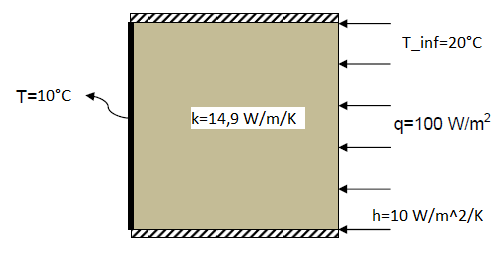
\includegraphics[width=0.9\textwidth]{calor1.png}
\caption{Esquema del problema a resolver}
\label{fig:calorP}
\end{figure}
\subsection{Soluci\'on anal\'itica}
Por las condiciones adiab\'aticas en los bordes superior e inferior se puede resolver el problema suponiendo que es unidimensional. La dependencia de la temperatura con la coordenada $x$ (sentido izquierda--derecha) es:
\begin{equation}
\frac{d^2T}{dx^2}+\frac{\dot{q}}{k}=0
\label{eq:calor1}
\end{equation}

Cuya soluci\'on es:
\begin{equation}
T(x)=-\frac{\dot{q}}{k}\frac{x^2}{2}+A\,x+B
\end{equation}

Donde $B=10\celsius$ y $A$ es igual a:
\begin{equation}
A=\frac{\dot{q}a\left( 1+\frac{h}{k}\frac{a}{2}\right) + |q|+h(T_{\infty}-B)}{h\,a+k}
\end{equation}
\subsection{Soluci\'on num\'erica}
Para implementar una solucion anal\'itica se discretiza el dominio de la siguiente manera:
\begin{figure}[h!]
\centering
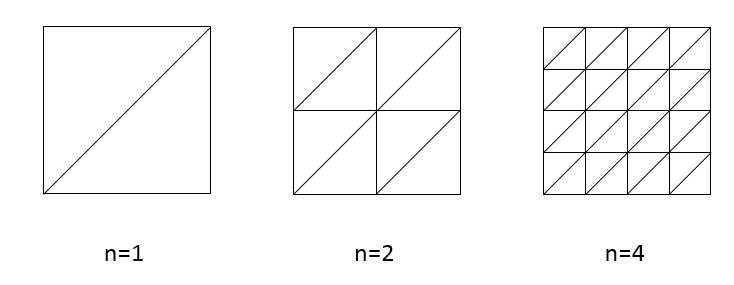
\includegraphics[width=\textwidth]{discret.png}
\end{figure}

Donde $n$ es igual a la cantidad de elementos ``cuadrados'' en los que se divide cada dimensi\'on. Luego cada elemento se subdivide en dos triangulares.

A esta discretizaci\'on se le aplica el m\'etodo visto en la parte te\'orica de la materia ``Ecuaci\'on de Poisson en 2-D'', para resolver el campo de temperatura.

\subsection{Resultados}
Una vez calculado el campo de temperatura se lo grafica en la Figura \ref{fig:c4}.
\begin{figure}[h!]
\centering
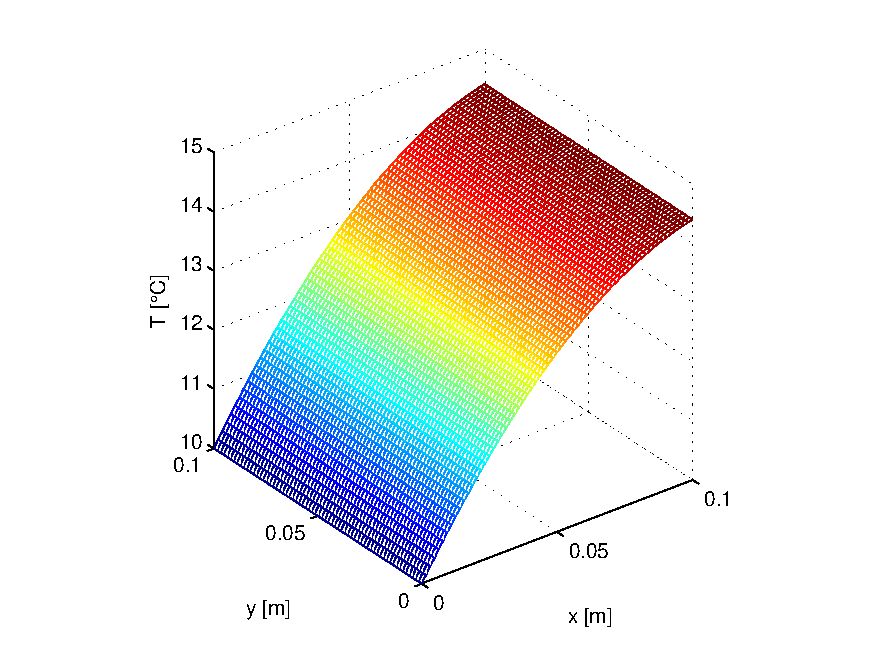
\includegraphics[width=0.8\textwidth]{calor4.pdf}
\caption{Campo de temperaturas en la geometr\'ia modelada.}
\label{fig:c4}
\end{figure}

A continuaci\'on se estudian los residuos del campo de temperatura. Los mismos son relativos al campo de temperatura obtenidos en la soluci\'on anal\'itica.

Primero se analiza el borde izquierdo. En la Figura \ref{fig:c2} se ven las curvas del residuo para diferentes valores de $n$. A medida que el valor de $n$ aumenta la curva del residuo se acerca a cero. Ademas se observa que para $y<50\,\milli\metre$ se comete un error por defecto, mientras que para $y>50\,\milli\metre$ se comete un error por exceso.
\begin{figure}[!ht]
\centering
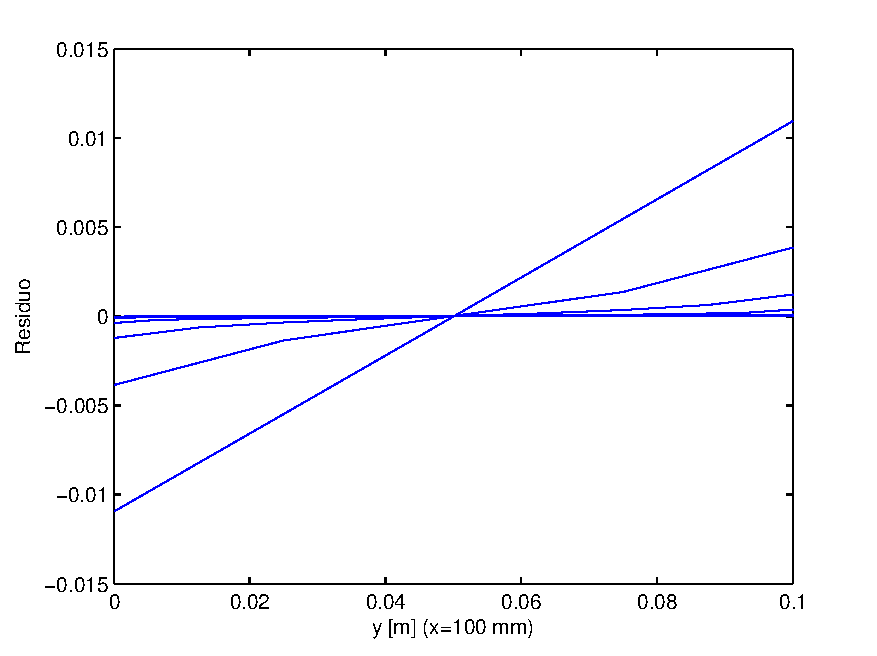
\includegraphics[width=0.9\textwidth]{calor2.pdf}
\caption{Se grafica el residuo en el borde izquierdo para diferentes valores de $n$. A medida que $n$ aumenta las curvas se acercan a cero.}
\label{fig:c2}
\end{figure}

A continuaci\'on se estudian los residuos en el borde inferior y en la linea media entre los bordes inferior y superior. En la Figura \ref{fig:c5} se grafican las curvas de residuos para cada valor de $n$ en el borde inferior. A medida que $n$ aumenta, el residuo disminuye. En la Figura \ref{fig:c1} se grafican las curvas de residuos para cada valor de $n$ en la linea media. En este caso a medida que aumenta $n$ el residuo aumenta. Esto se debe a que el residuo tiende a cero en esos nodos, pero \'este no puede ser menor que la precisi\'on del punto flotante. En ambas figuras se puede observar que el residuo es cero en $x=0$, ya que cumple necesariamente la condici\'on de temperatura fija en el borde izquierdo. 
\begin{figure}[!ht]
        \begin{subfigure}[ht!]{0.49\textwidth} 
	    \centering
	    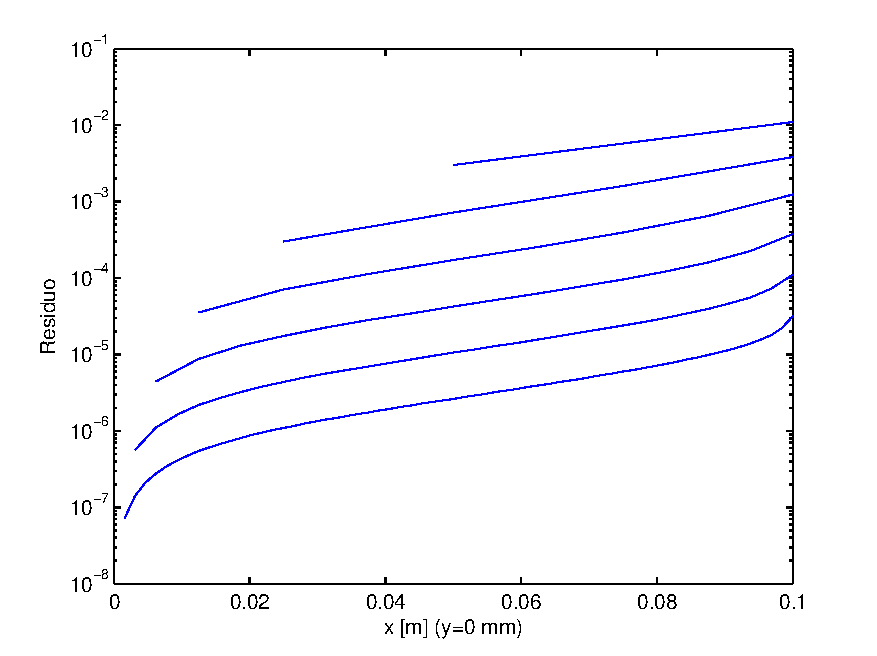
\includegraphics[width=\textwidth]{calor5.pdf}
	    \caption {}
	    \label{fig:c5}
	    \end{subfigure}
        ~
        \begin{subfigure}[ht!]{0.49\textwidth}
	    \centering
	    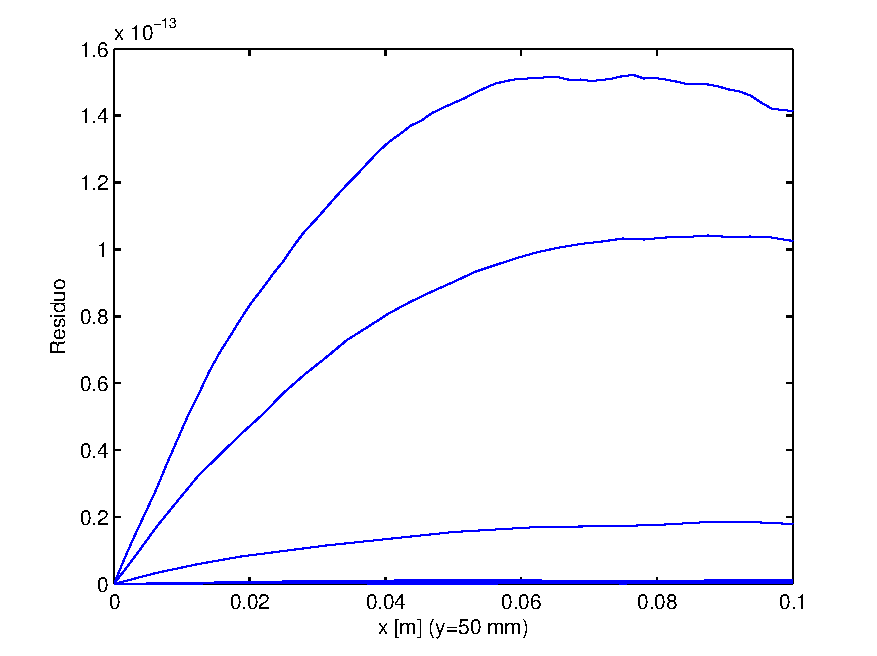
\includegraphics[width=\textwidth]{calor1.pdf}
	    \caption {}
	    \label{fig:c1}
	    \end{subfigure}
        \caption{Se grafican los residuos del campo de temperatura en (a) borde inferior y en (b) linea media entre los bordes inferior y superior}
\end{figure}
\newpage
A continuaci\'on se estudia el comportamiento del residuo en el punto de la esquina superior derecha a medida que se aumenta $n$ (o se disminuye la m\'inima distancia entre nodos $h$).
 
\begin{figure}[!ht]
\centering
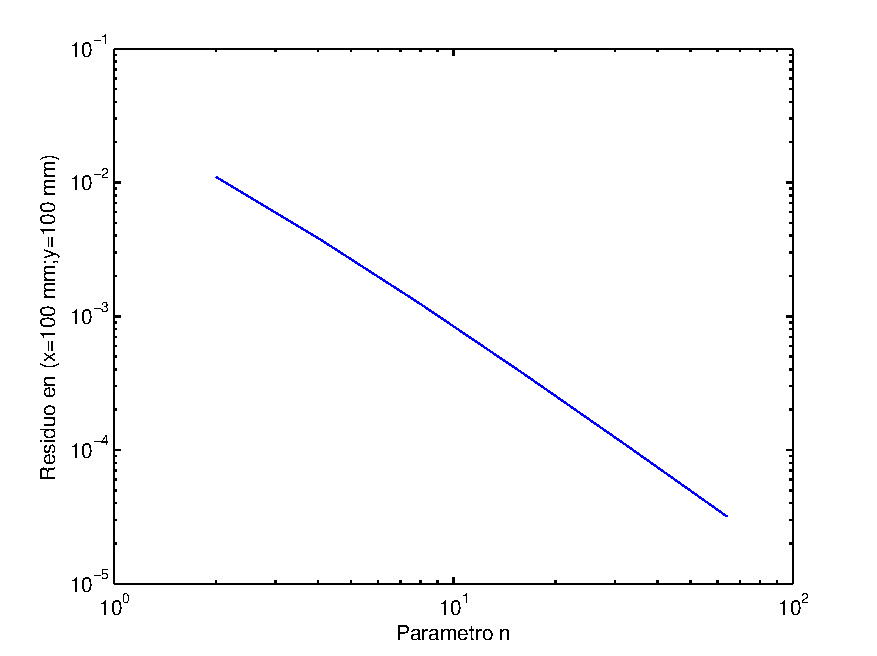
\includegraphics[width=0.9\textwidth]{calor3.pdf}
\caption{Gr\'afico del residuo en la esquina superior derecha en funci\'on de $n$}
\label{fig:c3}
\end{figure}

Por \'ultimo se realiza una estimaci\'on lineal sobre el gr\'afico log-log de la Figura \ref{fig:c3} resultando el residuo:
\begin{equation}
\epsilon\propto h^{1.6926}
\end{equation}